%!TeX root=Dissertation.tex
\subsection{Attack Detection Techniques}
Work done by Adi and Tripathi shows that even though HHTP/2, defined as RCF 7540, is a more  modern protocol, than that of HTTP/1.1, defined as  RCF 2616. Tripathi suggests that HTTP/2 has more threat vectors (\cite{tripathi2018slow}). Adi also notes that "The HTTP/2-standard states that if the host machine does not monitor resource usage, it exposes itself to a risk of a DoS attack" (\cite{Adi2015}).

The largest amount of research done into Low rate Dos attacks is by Erwin Adi, Zubair Baig, Chiou Peng Lam, and Phillip Hingston their work started in 2015 and they have 3 papers on this subject, the last of which was written in 2018. The majority of their work looked at using resource utilisation in order to detect Low bandwidth attacks. They set numerous tests to analyse the behaviours of victim machines when subject to Low rate Dos Attacks. 

The 2016 study carried out 4 varying investigations to analyse the behaviour of a victim machine when subject to large volume low rate DoS attacks. The researchers used a flood of windows PING and WINDOWS UPDATE frames to Simulate a Low-Rate DoS attack on a server, and demonstrated how legitimate HTTP/2 Flash Crowd could be launched to create a DoS scenario.  The team noted at the time of their 2016 investigation that there was no reported study to ascertain whether or not attack traffic could be concealed in a stealthy manor to appear as legitimate Flashcrowd traffic. The research concluded that the HTTP/2 protocol itself does not restrict the intensity of traffic generated, and that auxiliary mechanisms should be implemented for identifying volumes and patterns of network traffic. (\cite{Adi2016}) Trapathi stated as criticism in his 2018 study that neither the 2015 or 2016 studies completed by Adi's team managed to achieve a completed exhaustion of computational resource (\cite{tripathi2018slow}) Therefore it could be argued that Adi's research did not represent the full effect of a DoS attack, when looking into detail of the results from Adi's research, the figures quoted in Table 1 in the paper by Adi show depletion rates of between 88.39\% to 98.56\% (\cite{Adi2016}). Due to the ineffective depletion of the CPU the majority of his detection methods should be questioned as Trapathi points out....Even Erwin Adi himself points out that his methodology could potentially be flawed. Therefore Adi's proposed method for monitoring CPU depletion as a way to detect low rate bandwidth attacks could be fundamentally flawed. Adi's study was completed on a server with one single website and did not run any other background services for example, email, which would in theory add unpredictable CPU loads and make his detection method difficult to implement.

\begin{wrapfigure}{R}{}
\label{addie table}
    \centering
    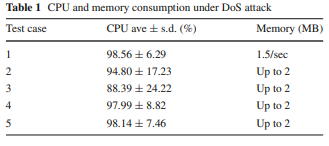
\includegraphics{Apdenix/adiTable.PNG}
    \caption{Table 1 from \cite{adi2017stealthy}}
    \label{fig:my_label}
\end{wrapfigure}
Although Adi's 2016 work looked at HTTP/2 it was noted in their later 2017 paper that 90\% of contemporary web servers up to the date of that study had not yet migrated to HTTP/2 from HTTP/1.x (\cite{adi2017stealthy}) At the time of this paper November 2019, HTTP/2 was used by 41.7\% of the top 10 million websites (\cite{w3techs}), as seen in figure \ref{web http2} below. 
\begin{wrapfigure}{L}{}
\label{web using h2}
    \centering
    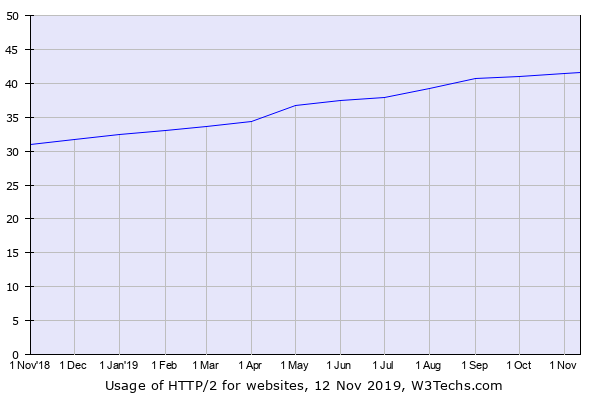
\includegraphics[width=88mm,scale=0.8]{Apdenix/HTTP2SITESgraph.png}
    \caption{Usage of HTTP/2 for Websites, 12 Nov 2019, W3Techs.com}
    \label{web http2}
\end{wrapfigure}This illuminates the pressing need for research into the assailability of the HTTP/2 protocol and consequent detection methods and fixes. 
 
Tripathi's 2018 study took a sample of websites and attempted to detect Low rate attacks by monitoring benchmarking and measuring the Chi squared (X\textsuperscript{\small2}) differential value between the expected and observed traffic pattern. Tripathi suggests this approach could detect attacks with high accuracy and may lead to further research to assess further HTTP/2 vulnerabilities thus potentially mitigating these threat vectors with fixes. Trapathi indicated that although his detection method for attack traffic was successful; if HTTP/2 traffic data is encrypted it must then be decrypted before submitting traces to the detector. He suggested that this could be easily achieved with the aid of an intercepting proxy before forwarding to the target website responsible for handling HTTP/2 requests. It must be noted that most large companies are utilising this strategy to intercept traffic coming into their local network. (\cite{tripathi2018slow}). 

Adi's 2017 work looked at some of the stealthier approaches that cyber attacks were using in order to bypass current detection methods. Adi and his team set up two models intended to simulate stealthy Low rate DoS attacks which they called 'bots'. The investigation aimed to model attacks whose traffic continually consumed the victims computing resource, while still being stealthy enough to yield some false alarms via the target servers' 'learning' mechanisms. Adi constructed the attack 'bots' with four core factors for experimentation, these were number of threads, number of window\_update, stealthy factor and delay between successive TCP connections. These two sets of Stealth models were tested against regular flash crowd traffic in an effort to differentiate the pattern. The experiment and subsequent analysis was successful in distinguishing a notable difference in the patterns of the number of packets carrying SYN flags per 1-second traffic instance between regular flashcrowd traffic and the simulated stealthy attacks. (\cite{adi2017stealthy}) Since Adi's work there appears to be an implementation of the methodology proposed in their paper. Cloudflare have been able to implement a defence mechanism against a SYN flood attack. The have created a program called 'gatebot' which monitors SYN packet packet requests and attempts to drop malicious SYN packets on the firewall layer (\cite{CFSYN}) the work does not refer to that of Adi's however the cloudflare implementation does appear to use similar concepts. At the  time of writing this seems to be the only documented attempt of blocking SYN attacks.